
%<!-- Titleseite -->
\thispagestyle{empty}

%%% redefine \maketitle
\renewcommand{\maketitle}{
	\begin{titlepage}
		\begin{center}
			\setlength{\parskip}{0pt}
			
			%	    \begin{flushright}
			%	    \colorbox{darkgray}{\color{white}{\Large \textsf{\@headerimg}}}
			%             \end{flushright}
			\begin{multicols}{2}
				\flushleft
				{Prof. Dr. Angelika Vetter\par}
				%{Seminar: Representative, direct and\\ cooperative participation in comparison\par}
				{Institute for Social Sciences\par}
				{Department of Political Systems \&\par}
				{Political Sociology}
				\begin{flushright}
					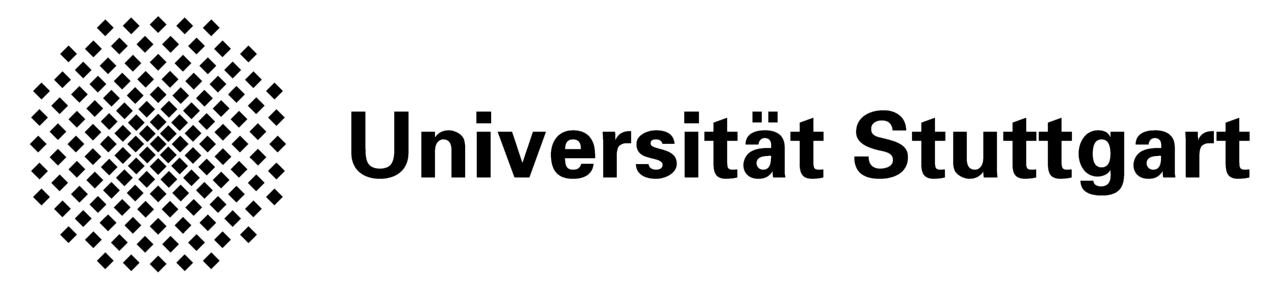
\includegraphics[width=7cm]{images/logo_stuttgart.jpg}
				\end{flushright}
			\end{multicols}
			\vspace*{2mm}
			\center
			{\LARGE {Seminar Paper} \par}
			
			\vspace*{10mm}
			
			
			{\fontsize{26}{38} {\bfseries Direct Democracy in Europe} \par}
			\vspace*{1mm}
			{ \Large A Cross-National Examination of the Link Between Direct Democracy and Satisfaction with Democracy in 31 countries}
			\vspace*{10mm}
			
			\begin{multicols}{2}
				\center
				Author: Fabio Votta, B.A.\\
				Email: \href{mailto:fabio.votta@gmail.com}{fabio.votta@gmail.com}\\
				Student ID: 2891518\\
				
				Author: Rosa Seitz, B.A.\\
				Email: \href{mailto:rosa.marie.seitz@gmail.com}{rosa.marie.seitz@gmail.com}\\
				Student ID: 2876533\\
			\end{multicols}
			
			
			\vspace*{5mm}
			
			
			
			
			
			\vspace*{5mm}
			{Date of Submission: 30.03.2018 \par} %\date{xxx}
			
		\end{center}
		\vspace*{2mm}
		\begin{abstract}
			\justifying
			\noindent This seminar paper seeks to investigate deliberation and its relationship to regime support across the world. This is accomplished by exploring the relevant literature and deriving hypotheses from it, which are subsequently tested by using survey data covering 113 countries and 306,047 individual respondents. Given that self-reported regime support is expected to be biased, a weight is applied to account for possible distortions of the data, though results are also reported for the unweighted variable due to the experimental nature of this weight. As this paper is the first known to the authors that examines the effect of deliberation on regime support in a cross-country design, the used deliberation measurement, the Deliberative Component Index from the “Varieties of Democracy”-Project, is examined in a thorough manner and analyses are conducted for its components as well. The analysis finds contradictory evidence for the proposed hypotheses. Deliberation seems to increase regime support first and foremost in democracies, the results in non-democracies and the complete sample are ambiguous and less robust. Furthermore, an exploratory mediation analysis is conducted, to test whether the macro-effect of deliberation on regime support is mediated through democratic performance evaluation on the individual level.  The findings of the analysis suggest that further studies in the field should investigate the relationship between deliberation and regime support as well as democratic performance evaluation in greater detail and find possible methods to remedy bias in self-reported regime support. Moreover, more sensible ways to measure deliberation on the country level are necessary, as it is highly correlated with democracy, although some interesting deviations could be found within the subsamples as well as in regards to the individual components. 
		\end{abstract}
	    \vspace*{2mm}
        \center		
		{\large {Seminar: Representative, direct andcooperative participation in comparison} \par}
		
	\end{titlepage}
}

%%% automated table of contents
\newcommand{\contents}{
	\newpage
	\thispagestyle{empty}
	\vspace{20mm}
	\tableofcontents
}



%%% Title page
\maketitle
\newpage
\contents
\clearpage
\listoffigures
\clearpage
\listoftables
\clearpage

%\clearpage
%
%%<!-- Inhaltsverzeichnisse -->
%\thispagestyle{empty}
%\setstretch{1.15}
%\tableofcontents
%\listoffigures
%
%\clearpage
%\setstretch{1.44}
%<!-- \onehalfspacing -->